\chapter{The Adapter Framework}

\section{Introduction}
\label{sec:adapter:intro}


Software components are self-contained entities with a well-defined interface and behavior. 
For two components to co-operate they must be \emph{integrated} through a compatible interface. 
The integration task also entails creating dependencies between the components, i.e. assigning objects to fields in order to communicate data.
The assignment operation requires the object and the assigned field are of a compatible \textit{type}.
When components are developed separately the compatibility is not a given. 
Therefore it should be, often manually, established through additional programming. 

The problem of incompatible interfaces is a common software engineering problem and a possible  solution is captured in the \emph{adapter pattern}~\cite{Gamma1995}.
The adapter pattern describes how to make two types compatible with each other. 
When an object makes a reference to a data value it requires a specific type, which we refer to as the \textit{target type}. 
Another object which represents the desired data and behavior but is an instance of the so-called \textit{source type}, different from the target type, is made compatible with an \emph{adapter}.
An adapter implements the methods of the target type by invoking methods defined in the source type, thereby establishing compatibility.
There are two types of adapters; class adapters and object adapters.
Class adapters use multiple inheritance to subclass both the source and the target types.
Object adapters wrap the source object and subclass the target type; it implements the target methods by invoking the methods of the source object.
An adapter introduces a level of indirection between the types whose interfaces are incompatible with each other.

There are some issues attached to the traditional adapter pattern.
A class adapter is easily implemented with a language that supports multiple inheritance. 
Developers using single inheritance programming languages need to use workarounds to achieve the same effect.
For example in Java multiple inheritance is simulated with the usage of interfaces since a class can implement multiple of them. 
In order to inherit from two concrete types using Java, we need to extract the interface of one of the types and add this interface to the list of super-interfaces. 
However, we don't always have control over source code which would allow these operations. 


The implementation of the object adapter pattern is more flexible, since it only needs to inherit from the target type. 
However the adapter class is an additional type that is introduced to the source code. 
Hence the adapter definitions themselves are dependent on other types; they also need to ne updated when the source or the target interface is altered, thus requiring additional maintenance.
 
The integration code contains a direct reference to the adapter type instead of just the source and the target types, which introduces additional maintenance efforts. 
Another problem is related to the \emph{reuse of adapters}.
The developer may not possess the knowledge of which adapter is suitable for the adaptation task at hand.
This is a problem when adapters are not planned to be reusable and documented poorly. 
Then one has to search the type hierarchy to find the classes implementing the target type, then among these classes the suitable adapter has to be found. 
The developer may even have to identify if the class she found is indeed an adapter class if it is not clear from the naming.
This is an ad-hoc process that is error-prone as well as time consuming.


So far we have established that integrating two separately developed components requires making their interfaces compatible and assigning object values to the appropriate field thereby building the necessary dependencies.
The latter is implemented in the \emph{glue code}.
In component-based design loose-coupling is an important principle.  
Dependency injection (DI) (cite fowler) is a lightweight method for keeping modules loosely coupled by delegating the creation of concrete objects to so-called \emph{injectors}. 
This approach allows a creating loosly coupled dependencies. 
When using the adapter pattern, the injection specification is coupled to the adapter implementation.
This means during development time the adaptation and the binding tasks are not independent of each other; the developer that is writing the glue code should be aware of the adapters that are available to her.

Let us summarize the problems we have identified above:
\begin{enumerate}[{P}-1]
\item Implementation of the adapter pattern can be hindered by programming language properties.
\item Adapter pattern introduces additional dependencies, which increases maintenance efforts.
\item Reusing adapters require additional knowledge and effort from the side of the developer to be used properly.
\item The glue code contains dependencies to the adapter classes, which hinders loose coupling.
\end{enumerate}

In light of the issues discussed, we have devised the requirements below. The first three requirements refer to a specific problem in the above itemization. The last two requirements are concerned with the binding.

\begin{enumerate}[{R}-1]
\item It must be possible to implement adapters without inheritance. (P-1)
\item The adaptations must be performed without creating dependencies to specific adapter classes. (P-2)
\item Adapters must be found automatically given a source object and a target type. (P-3)
\item Glue code must not contain references to concrete adapters; it must be possible to implement these separately. (P-4)
\end{enumerate}

In order to satisfy these requirements we have designed the \zamk framework, which unites dependency injection with \emph{under-the-hood} adaptation logic.
For our framework we do not employ the traditional adapter pattern but we have created the concept of \emph{converters}, which are user-defined classes that do not have to inherit from a target type to realize the adaptation.
\zamk comes with its own dependency injection mechanism that is used with a designated domain-specific language called \gluer. 
The dependency injection logic is intertwined with the adaptation logic which uses the conversion registry to perform automated adaptation between source and target types. 
We automate the adaptation process by exploiting the type hierarchies and provide checks and context-relevant messages for correct integration. The details of the framework will be explained throughout the chapter.

\subsection{Motivating Example}
\label{sec:adapter:motiv}

In the previous section we have identified the problems attached to the traditional adapter pattern\footnote{Throughout this chapter, the term adapter pattern will refer to the object adapter pattern. References to the class adapter pattern will explicitly include the term class.} and we have come up with requirements for a solution that would remedy these problems. In this section we will illustrate the said problems with an example.
Assume we have a plot drawing software which uses the Cartesian coordinate system to represent the points in the plot. 
The software includes a data component which contains a class called \lstinln{Cartesian} which has two fields \lstinln{x, y}, that represents the values on the x-axis and y-axis respectively. 
This class also includes getters and setters for these fields (\lstinln{Component1} in Figure~\ref{fig:components}).
A new requirement is received which states that the software must also support polar coordinates, and the user must be able to view plot points in a selected view (\lstinln{Cartesian} or \lstinln{Polar}). 

In order to support polar coordinates, a new component which contains classes to represent such data is introduced (\lstinln{Component2} in Figure~\ref{fig:components}). The class \lstinln{Polar} contains two fields \lstinln{r} representing the radius and \lstinln{theta} of type \lstinln{Angle}. This component is to be integrated with the \lstinln{Cartesian} component. 
Consider we want to integrate both components using the traditional adapter pattern. 
It should be possible to obtain the \lstinln{Polar} representation of any \lstinln{Cartesian} object by using an \emph{adapter}.
This solution is discussed in the following.

\begin{figure}
\centering
\begin{tikzpicture}[scale=0.7, transform shape]

\begin{umlpackage}[x = 0, y = 0]{Component1}

\umlclass{Cartesian}
{
	x: double \\
	y: double \\
}
{
	
}

\end{umlpackage}

\begin{umlpackage}[x = 6, y = 0]{Component2}

\umlclass[x = 0, y= 0]{Polar}
{
	r: double \\
	theta: Angle \\
}
{
	
}

\umlclass[x = 4, y= 0]{Angle}
{
	value: double
}
{
	+getSin() : double \\
	+getCos() : double
}

\end{umlpackage}



\end{tikzpicture}
\label{fig:components}
\caption{UML diagram for the two components}
\end{figure}

An abstract view of the traditional object adapter pattern is shown in Figure~\ref{fig:oapattern}. The adapter pattern relies on inheritance and adds a level of indirection between the \lstinln{Client} and the \lstinln{Target}. The application of this pattern to the example case requires creating a Cartesian to polar adapter (\lstinln{Cartesian2PolarAdapter}) which takes a \lstinln{Cartesian} object as an \emph{adaptee} and extends the \lstinln{Polar} class to override its methods (Figure~\ref{fig:objadapter}). An implementation for this adapter is given in listing~\ref{lst:objadapterlst}.


\newsavebox{\cartesiantopolar}
\begin{lrbox}{\cartesiantopolar}
\begin{lstlisting}
public class Cartesian2PolarAdapter extends Polar{
	Cartesian adaptee;
	public Cartesian2PolarAdapter(Cartesian c) {
		this.adaptee = c;
	}
	public double getR()
	{
		return Math.sqrt(Math.pow(adaptee.getX(), 2) + Math.pow(adaptee.getY(), 2)));
	}
	public Angle getTheta()
	{
		return new Angle(Math.atan(adaptee.getY()/adaptee.getX())));
	}
}
	\end{lstlisting}
\end{lrbox}

\newsavebox{\cartesiantopolaraop}
\begin{lrbox}{\cartesiantopolaraop}
\begin{lstlisting}
public aspect Cartesian2PolarAdapter {

	declare parents: Cartesian extends Polar; ~\label{lst:line:it}~

	public double Cartesian.getR()
	{
		return Math.sqrt(Math.pow(this.getX(), 2) + Math.pow(this.getY(), 2));
	}
	
	public Angle Cartesian.getTheta()
	{
		return new Angle(Math.atan(this.getY()/this.getX()));
	}
}

	\end{lstlisting}
\end{lrbox}


\begin{figure}
\centering
\subfloat[Abstract view of the object adapter pattern]{

\begin{tikzpicture}[scale=0.5, transform shape]

\umlemptyclass{Client}
\umlclass[x = 4, y = 0]{Target}{ 
 
  }{ 
  + Request()
} 

\umlclass[x = 8, y = 0]{Adaptee}{ 
 
  }{ 
  + SpecificRequest()
}


\umlclass[x = 6, y = -3]{Adapter}{ 
  +adaptee : Adaptee
  }{
  + Request()
}

\umlinherit{Adapter}{Target}
\umluniassoc{Client}{Target} 
\umlaggreg{Adapter}{Adaptee}

  \end{tikzpicture}

\label{fig:oapattern}
}
\hfill
\subfloat[Concrete view of the object adapter for the example case]{
\begin{tikzpicture}[scale=0.5, transform shape]

\umlemptyclass{Client}
\umlclass[x = 4, y = 0]{Polar}{ 
 
  }{ 
  + getR() \\
  + getTheta()
} 

\umlclass[x = 8, y = 0]{Cartesian}{ 
 
  }{ 
  + getX() \\
  + getY()
}


\umlclass[x = 6, y = -3]{Cartesian2PolarAdapter}{ 
  +adaptee : Cartesian
  }{
  + getR() \\
  + getTheta()
}

\umlinherit{Cartesian2PolarAdapter}{Polar}
\umluniassoc{Client}{Polar} 
\umlaggreg{Cartesian2PolarAdapter}{Cartesian}

  \end{tikzpicture}

\label{fig:objadapter}
}
\vfill
\subfloat[The implementation for the \lstinln{Cartesian2PolarAdapter}]
{\usebox{\cartesiantopolar}
\label{lst:objadapterlst}}
\caption{The diagram of the object adapter and the corresponding Java implementation}
\end{figure}

A convenient implementation of the adapter pattern requires a lot of boilerplate code. 
An improvement over this implementation is proposed by  Hannemann and Kiczales~\cite{hannemann:oopsla02}. 
In this study they propose a re-usable implementation to the class adapter pattern using inter-type declarations. 
According to the auxiliary code they provide with this study, they propose the adaptee class should subclass the target class, which results as the diagram shown in Figure~\ref{fig:hkaop}.
For our example case the \lstinln{Cartesian} class will directly have to subclass the \lstinln{Polar} class and implement its method using its \lstinln{x, y} field values. This is depicted in the aspect shown in Listing~\ref{lst:objadapteraoplst}.
The inter-type declaration on line~\ref{lst:line:it} declares the inheritance relation and the subsequent method implementations are woven into the \lstinln{Cartesian} class.

\begin{figure}
\centering
\subfloat[Abstract view of the object adapter pattern with inter-type declarations]{
\begin{tikzpicture}[scale=0.6, transform shape]
\umlemptyclass{Client}
\umlclass[x = 4, y = 0]{Target}{ 
 
  }{ 
  + Request()
} 

\umlclass[x = 4, y = -3]{Adaptee}{ 
  }{ 
  + SpecificRequest() \\
  + Request() 
}
\umlinherit{Adaptee}{Target}
\umluniassoc{Client}{Target} 
\end{tikzpicture}
\label{fig:hkaop}
}
\hspace{20pt}
\subfloat[Concrete view of the aspect-oriented adapter pattern for the example case]{
\begin{tikzpicture}[scale=0.6, transform shape]
\umlemptyclass{Client}
\umlclass[x = 4, y = 0]{Polar}{ 
 
  }{ 
  + getR() \\
  + getTheta()
} 

\umlclass[x = 4, y = -3]{Cartesian}{ 
  }{ 
  + getX() \\
  + getY() \\
  + getR() \\
  + getTheta 
}
\umlinherit{Cartesian}{Polar}
\umluniassoc{Client}{Polar} 
\end{tikzpicture}
\label{fig:hkaopex}
}
\vfill
\subfloat[The implementation for the \lstinln{Cartesian2PolarAdapter} in AspectJ]
{\usebox{\cartesiantopolaraop}
\label{lst:objadapteraoplst}}
\caption{The diagram of the object adapter and the corresponding Java implementation}
\end{figure}

The obvious problem with this implementation is that, since \lstinln{Polar} is a concrete type, it would quickly become unusable due to Java's single inheritance. 
Another limitation comes from the semantics of inter-type declarations. 
Only \emph{sibling} types, i.e. types which share a parent class, can be used in an inter-type declaration. In this example both classes' super-type is \lstinln{Object}, which allows us to use the inter-type declaration. 

Up to now, we have explained the issues related to the implementation of adaptation concern, we also need to bind the newly added component to our application.
In order to bind the polar coordinates into our plotting software, we need to alter some code. 
According to the selection made in the GUI, the information box should display the coordinate value in the correct format. 
An example for the integration code is given in Listing~\ref{lst:integration}.
On line~\ref{lst:integration:adapt} we see an explicit reference to the class \lstinln{Cartesian2PolarAdapter}; this adapter is introduced at the beginning of the section in listing~\ref{lst:objadapterlst}.
Referring to a low-level implementation type hinders software evolution because we need to change code when another adaptation should be used. 
The other issue is that in order to reuse existing adapters, the developer has to have knowledge about these adapters, or she needs to search to see if a suitable one exists. 
The explicit reference on line~\ref{lst:integration:adapt} is also a disadvantage for the binding process since how the \lstinln{Polar} field is initialized is fixed with this reference.


\begin{lstlisting}[float, caption={The integration of Polar coordinates}, label={lst:integration}]

public void viewPointValue(Point selected)

	if(GUI.format == CARTESIAN)
		GUI.createNewValueBox(selected.loc(), selected.getCoordinates().toString());
	else if(GUI.format == POLAR)
	{
		Polar p = new Cartesian2PolarAdapter(selected.getCoordinates()); ~\label{lst:integration:adapt}~
		GUI.createNewValueBox(selected.loc(), p.toString());
	}
}
\end{lstlisting}

In this section we have used the plotter example to illustrate the problems we have identified in Section~\ref{sec:adapter:intro}. 
Firstly we have described how programming languages can affect the implementation of the adapter pattern by using Java and AspectJ (P-1). 
Secondly we have shown the disadvantages of introducing adapter dependencies in the integration code, by using the introduction \lstinln{Polar} view extension to the plotter software (P-2).
Thirdly, using the same example, we have discussed why the developer needs adapter specific knowledge and how it slows down the integration process (P-3). 
Lastly, we have discussed the disadvantage of having an explicit dependency in the glue code.


\section{Approach}
\label{sec:adapter:approach}
In this section we will explain the details of the \zamk framework which is designed according to the requirements specified in Section~\ref{sec:adapter:intro}. 

\zamk is a development framework specifically tailored for reusable adapters and adapter-aware dependency injection. 
It offers a new and a light-weight way of defining adapters; these light-weight structures are called \emph{converters}. 
Converters contain the logic that is used to convert one type to another. 
Typically this logic defined how an object of a target type can be initialized using the values provided by an object of a source type (e.g. calculating the polar coordinate values from Cartesian values). 
Converters are provided by the developer and they do not need to use sub-class any of the types to implement adaptations. Converter classes are stateless. 
\zamk runtime is responsible for finding the correct converter, given a source and a target object. 
This means the only additional dependency we have to include in the implementation is the \zamk runtime API. 
Since the user does not have to refer to specific adapters, \zamk allows separation of adaptation and binding concerns during integration.
\zamk also comes with its own binding language, so-called \gluer, which uses dependency injection under-the-hood. 
\gluer~ is a domain-specific language and its declarative nature allows compile-time checks.
The user is flexible in how she chooses to use \zamk, she can either use the \gluer language or she can call the runtime API directly. 
Integration using \zamk also helps separating the binding concern and the adaptation concern from each other.  

\begin{figure}
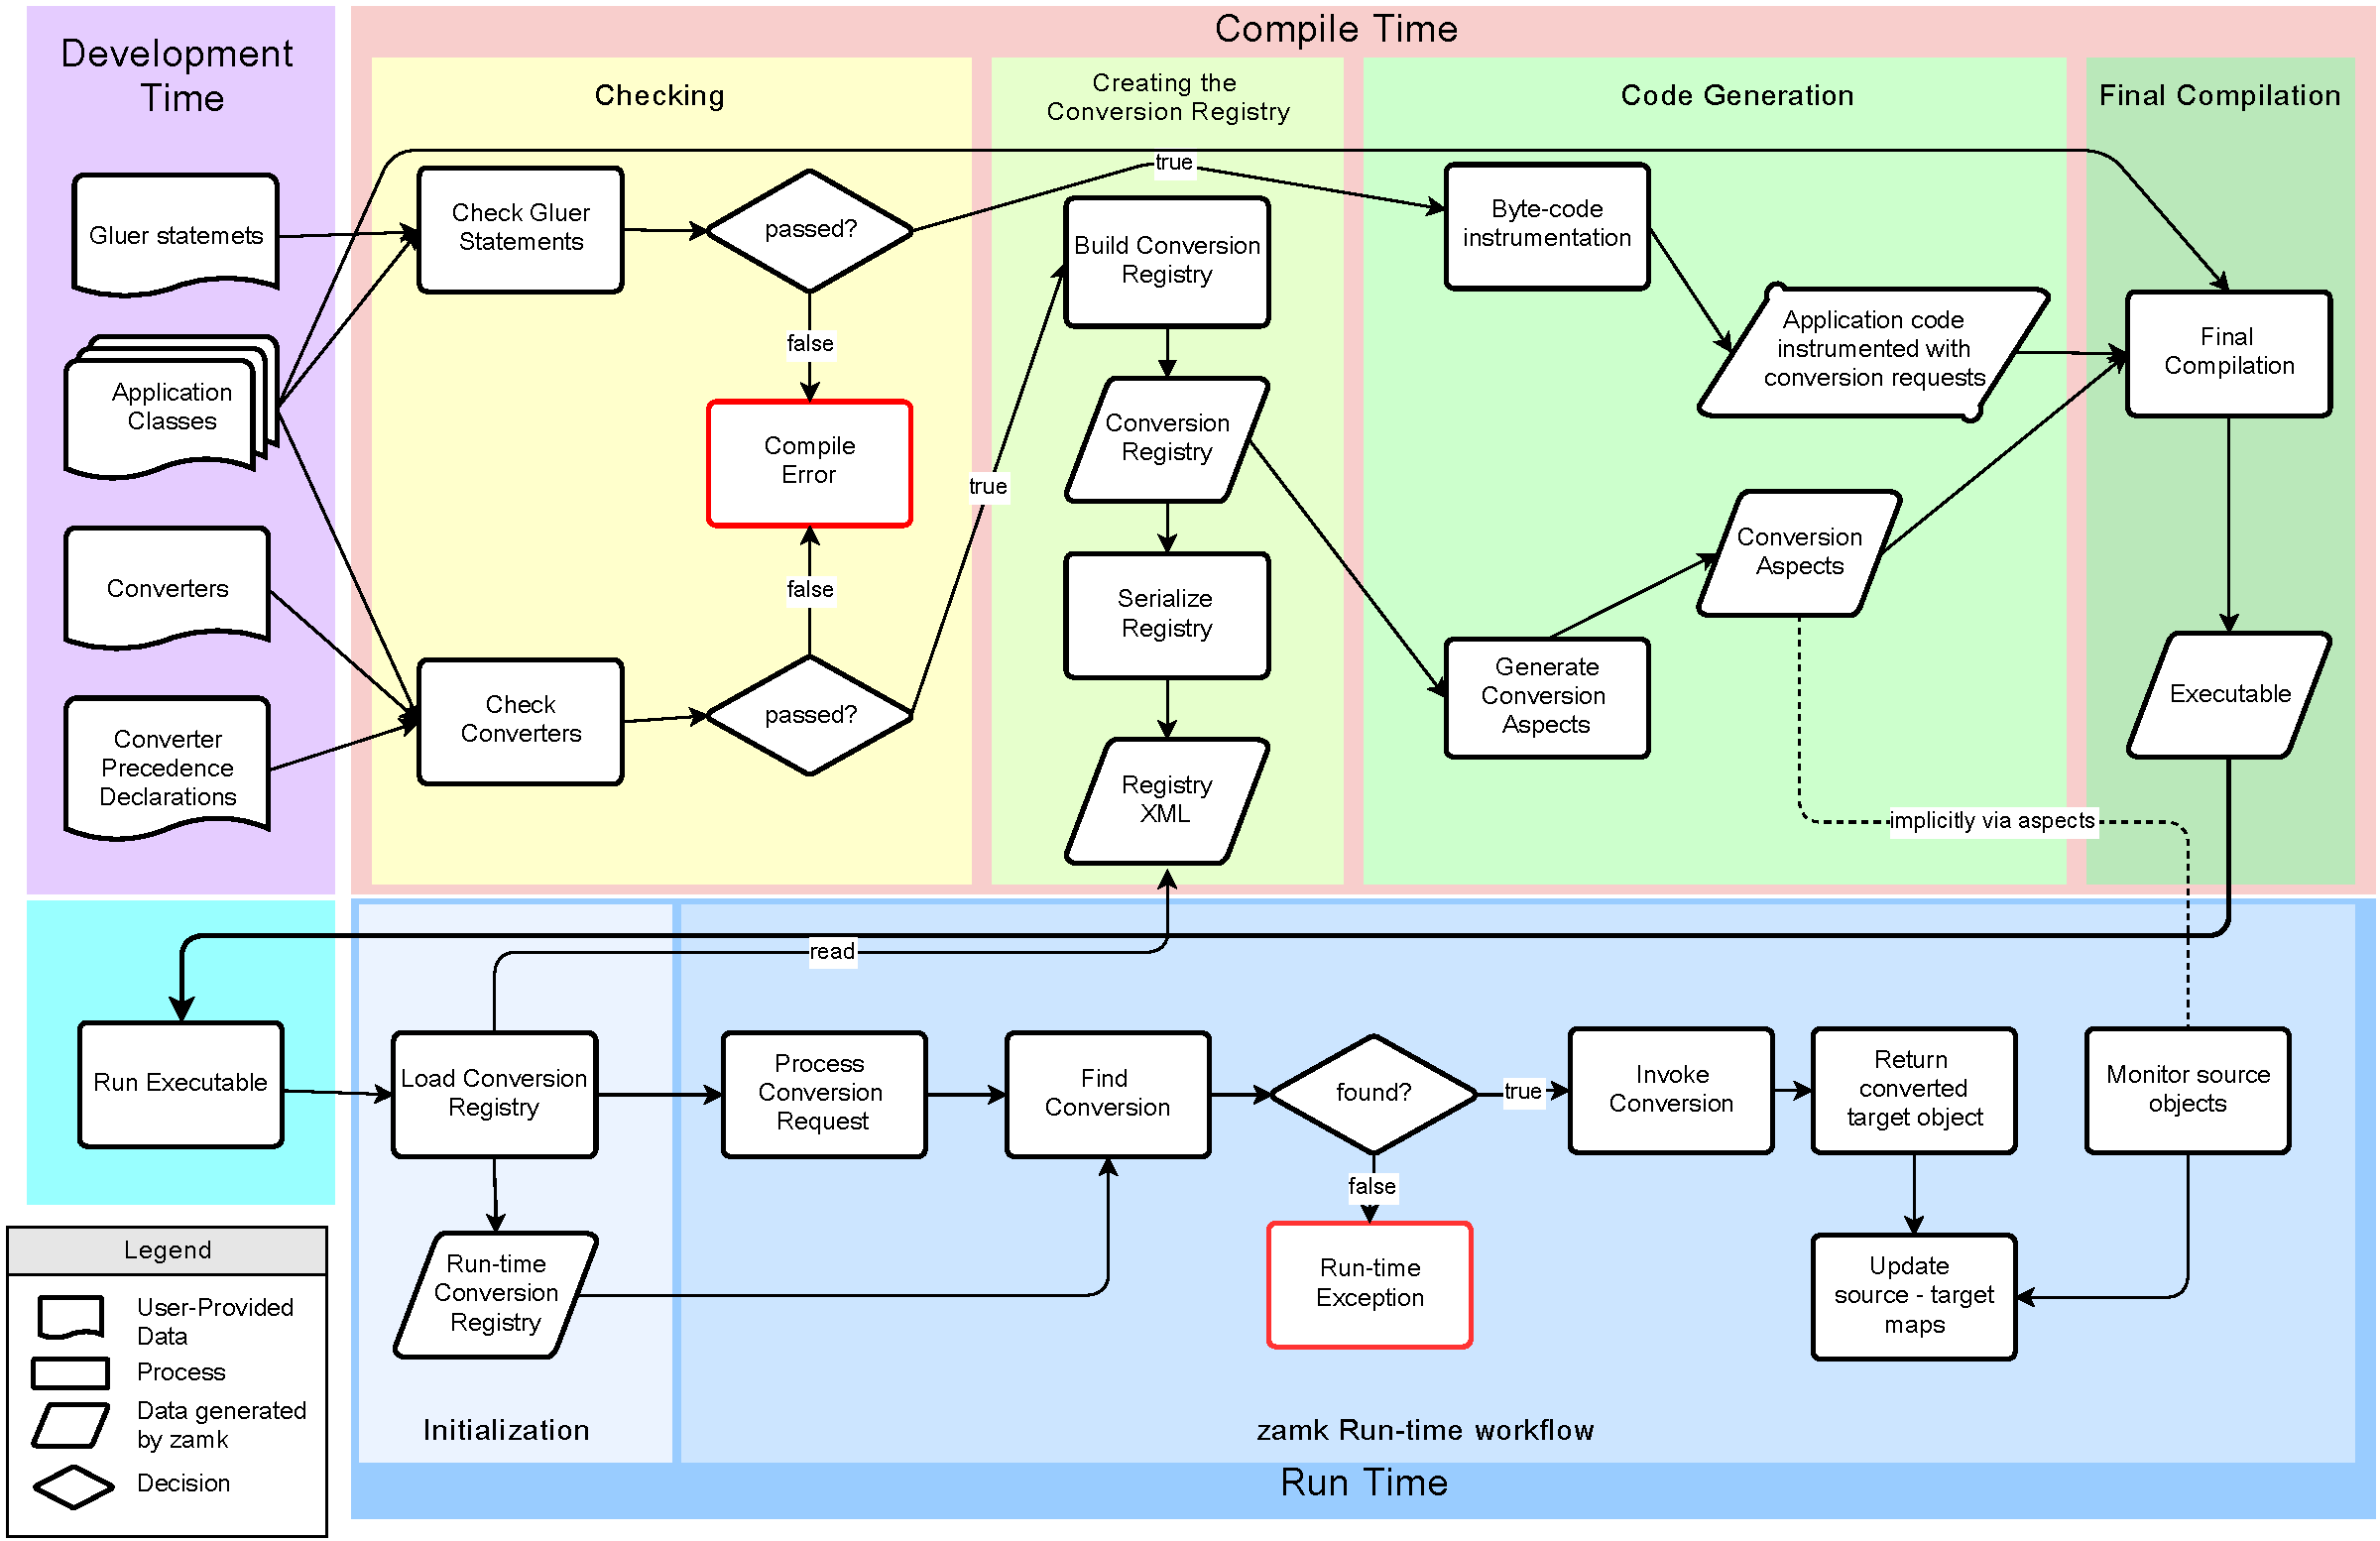
\includegraphics[height=\textwidth, angle=90]{chapteradapters/bigpicture.pdf}
\caption{An overview of the \zamk framework}
\label{fig:framework}
\end{figure}

Figure~\ref{fig:framework} shows an overview of the stages that are necessary to perform an integration using \zamk.
\zamk requires user-defined input to perform an integration.

\paragraph{Development Time}
The goal of the \zamkph{development time} is to provide the necessary input to \zamk. 
In the figure we show four inputs that are fed to the \zamk compile-time; they are (in the order shown in the figure):

\begin{description}
\item{\gluer files}: Gluer files contain the \gluer statements that define which objects are going to be injected to which fields. \gluer statements are used to generate conversion requests, which are \zamk API calls that trigger the \zamk adaptation work-flow. The \gluer language is discussed in Section~\ref{sec:adapter:gluer}. 
\item{Application Classes}: These classes are scanned to retrieve information for integration. The retrieved information is used in checking. Also application classes are instrumented with conversion requests that are derived from \gluer statements. 
\item{Converters}: Converters contain methods necessary to convert one type to the other. They are annotated in order to be registered by \zamk. 
These are discussed in Section~\ref{sec:adapter:converter}.
\item{Converter Precedence Declarations}: These are used to resolve conflicts when more than one conversion is found for a specific request. In this case the conversion which is contained by the converter class that has the higher precedence is used. 
\end{description}

It is also possible to write plain Java code that calls the \zamk API directly.
However these statements are not processed during compile-time. 
That is why we do not list them as compile-time inputs. 
During the \zamkph{final compilation} phase, they are compiled with all the code that is provided by the user and generated by \zamk.

\paragraph{Compile Time}
The goal of the compile-time stage is to check the provided input and generate the necessary code using the information derived from the input.
Once the input is provided, the \zamk compile-time work-flow starts. This work-flow is composed of the following sequential phases. The descriptions below follow the same structure and the order as in upper-half of the Figure~\ref{fig:framework}. 

\begin{description}
\item{\zamkph{Checking}}: There are two checkers; one responsible for checking the \gluer files and the other for converter classes. The gluer checker performs the syntax checking; it also checks if the references made in the \gluer statement actually exist in the application code. The converter checker performs type checking and well-formedness checking. If any of these checks fails, a compile-error is produced. 
\item{\zamkph{Conversion registry}}: When the converter checking is finished without any problems, \zamk builds a conversion registry\footnote{One converter class may include multiple conversions} in the form of a data structure to be used in the next step of compile-time work flow: \zamkph{code generation}. Also during this phase the conversion registry data structure is serialized in XML format creating the registry XML. 
\item{\zamkph{Code Generation}}: This step consists of two separate generation processes. Byte-code instrumentation is responsible for inserting \zamk conversion requests to the places indicated as the binding points defined in the \gluer statements, i.e implementing the dependency injection.
The conversion registry that is created in the previous step is used to generate the \emph{conversion aspects}.
The conversion aspects are responsible for monitoring the source objects which are associated with a target object. 
\item{\zamkph{Final Compilation}}: When the compile-time work flow is complete a final compilation step is performed, which makes sure the instrumented application classes and the generated files do not contain any errors. At the end of this step we obtain a \zamk run-time ready code, in this figure we assume the final compilation product is an executable.
\end{description}
 
The \zamk compile time produces two outputs; registry XML which will be loaded during \zamkph{run-time initialization} and the compiled code of \zamk generated classes and application classes. 


\paragraph{Run-time}
During run-time \zamk processes conversion requests.
\zamk run-time consists of two parts, a one time \zamkph{initialization} and a \zamkph{run-time work flow} which is executed for every conversion request (
lower-half of Figure~\ref{fig:framework}). 

\begin{description}
\item{\zamkph{Initalization}}: The \zamk run-time starts with an initialization step, which loads the conversion registry that is serialized during runtime. 
The loading process produces a data structure called run-time conversion registry, which is used by the run-time work flow to locate conversions.
\item{\zamkph{Run-time workflow}}: The compiled program contains \zamk conversion requests which trigger the conversion finder. 
A conversion request contains the source object and the desired target type to which the source object should be converted. 
The \emph{find conversion} process searches for the correct conversion by using the type information included in the conversion request. 
If a suitable conversion cannot be found, \zamk produces a run-time exception indicating the error. 
When a conversion is found, one of two things can happen. 
If the requested conversion was never performed before for the given source object and the target type, the suitable conversion method is invoked and an object of target type is created. 
This pair of objects, provided source object and the associated target object, is referred to as a source--target pair. 
Alternatively, \zamk may find that a request to the same target type was processed before with the given source object. 
In that case the existing target object is retrieved and returned. 
\end{description}


\subsection{Conversions Instead of Adapters}
In the traditional adapter pattern, the adapter class has an adaptee; if this adaptee's value is changed, it directly affects the return values of the methods that are implemented by the adapter.
In order to eliminate the dependency to the adapter type, we have created the notion of conversions. 
Conversions are defined in user-provided converter classes. Conversions simulate adaptation as a one-time conversion and a series of updates during an objects life-cycle. 

A conversion consists of two parts, the first part consists of two user-defined methods: a convert and an update method. 
The second part is an \emph{aspect}, so-called conversion aspect, generated by \zamk which contains a hash-map of source (adaptee) and target objects. 
The conversion aspect is generated during compile-time\footnote{Please refer to the code generation step of Figure~\ref{fig:framework}}. 
The responsibility of this aspect is to monitor the source (adaptee) objects and update the target objects if a source object changes. 
The update operation is performed by calling the user-defined update method.

In Figure~\ref{fig:conv1} the first step of the conversion process is shown. 
A new conversion requested by giving a source object and a target type. 
In the traditional adapter pattern this source object is the adaptee and an adapter which is a subtype of the target type is instantiated that aggregates this source object. 
In our conversion process this source object is passed onto the convert method of an appropriate conversion (automatically found by the framework, section~\ref{sec:adapter:find}) and this method returns the corresponding target object, which is initialized according to the values provided by the source object. 
When a new target object is created, the \zamk runtime registers the source-target pair in a hashmap. 
This hashmap represents the \emph{has-a} relationship between the adapter and the adaptee. 

Once a target object is linked to a source object, they are kept synchronized. 
This is ensured by the generated conversion aspect. 
The conversion aspect monitors the events which change the source objects, when such an event is encountered it retrieves the corresponding target object. 
Then it triggers the \emph{update} method in the converter class to update the target object that is linked to the changed source object.

\begin{figure}
\subfloat[A new adaptation request]{
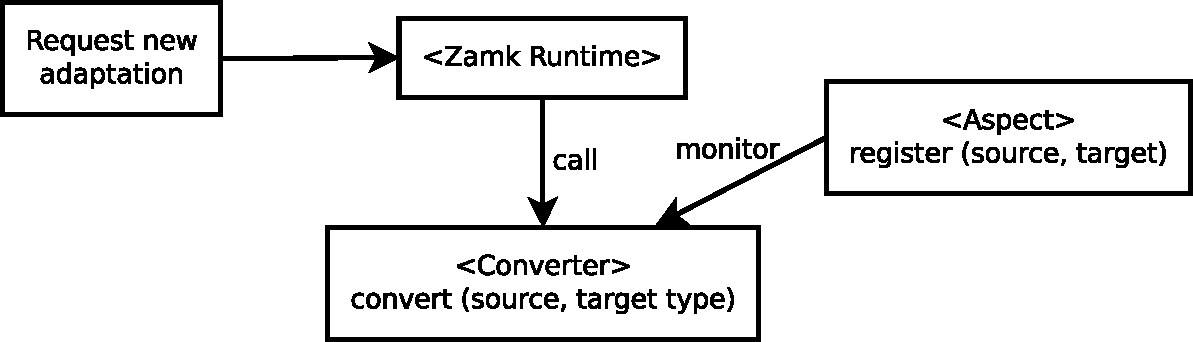
\includegraphics[width=0.45\textwidth]{chapteradapters/conv1.pdf}
\label{fig:conv1}
}
\subfloat[Keeping source and target objects synchronized]{
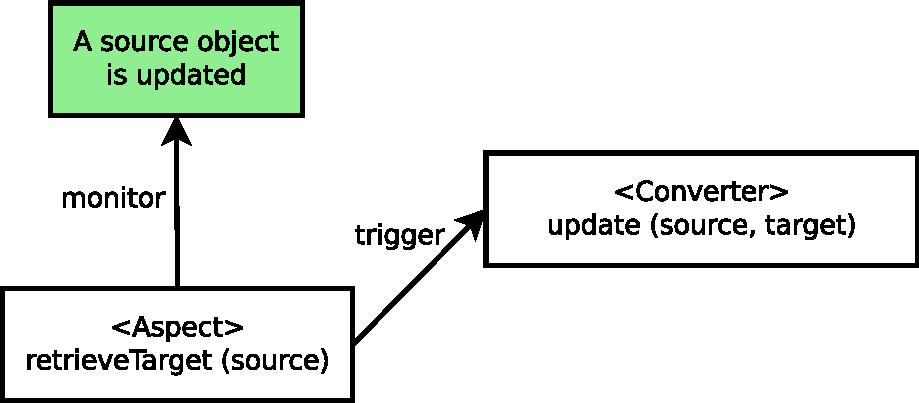
\includegraphics[width=0.45\textwidth]{chapteradapters/conv2.pdf}
\label{fig:conv2}
}
\end{figure}

In this method of adaptation, there is no need to create an intermediate adapter type.
The converter directly creates an object of the target type and keeps it up-to-date. 
As we will explain in section~\ref{sec:adapter:compile}, the user only has to define a conversion in a converter class. 

%Our decomposition provides a uniform way of implementing adapters.


\subsection{Compile-time}
\label{sec:adapter:compile}

In this section we will explain the elements and modules that are involved during the compile-time of the framework. In figure~\ref{fig:ctwf} a simplified version of the compile-time work-flow is shown.
In this figure we have numbered the steps taken in the compile-time, since they are performed sequentially.


As mentioned before, the developer is responsible with providing converters that are specific to her application. The converters are required to adhere to a specific structure, which is discussed in section~\ref{sec:adapter:converter}. 
The correctness of the converters are checked by the process \textsf{Check Converters}, in the \textsf{Checking} step. 
All of the processes in this step take the application classes as input, since the checking operation uses these classes to investigate the existence of the dependencies. 
\gluer files are checked by the \textsf{Check Gluer Statements} process. This process, the related processes and the input and outputs are shown in dashed style, since providing \gluer files is an optional step. 
As mentioned before it is also possible to call \zamk API directly from Java. 

Once the provided input is checked and proved to be error-free, the checked converter classes are input to the \textsf{Build Conversion Registry} process, inside the \textsf{Creating the Conversion Registry} step. 
The processes included in this step are also numbered, since the \textsf{Serialize Registry} process requires the conversion registry data structure produced by the \textsf{Build Conversion Registry} process.

The conversion registry data structure is also passed to the third step \textsf{Code Generation}, which contains two processes. First one is the optional process \textsf{Byte-Code Instrumentation}, which takes the checked \gluer files as input. 
This step is not performed if no \gluer files are provided.
Second one is the \textsf{Generate Conversion Aspects} process, which takes the conversion registry as input and outputs the conversion aspects. 

The fourth and the final step is the compilation of all code that is generated by \zamk and provided by the developer. 

\begin{figure}
\centering
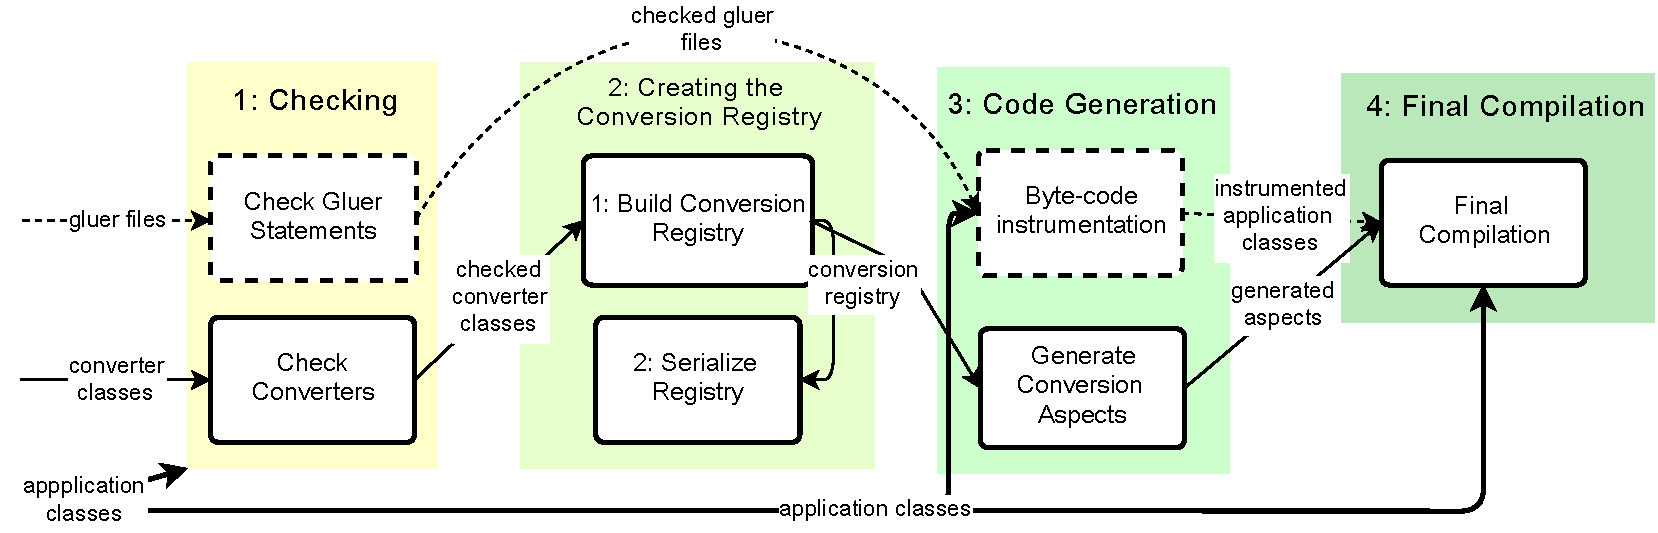
\includegraphics[width=\textwidth]{chapteradapters/compiletime.pdf}
\caption{The compile-time workflow and dataflow of \zamk}
\label{fig:ctwf}
\end{figure}

\subsubsection{Gluer DSL}
\label{sec:adapter:gluer}
The \gluer language is a concise DSL that is designed to declare dependencies between fields and objects. 
We have developed the \gluer language to offer an external, non-intrusive way of declaring bindings. 
Essentially \gluer is an external dependency injection declaration language which creates the objects to be injected and is connected to an adaptation logic which can process the created objects before the  injection happens.
A \gluer program is stored in a file with the extension `.gluer'.

\paragraph{Syntax and Semantics} We chose the keyword \lstinln{glue} instead of \lstinln{inject} since \gluer does more than dependency injection. 

The syntax of the \gluer statements is defined as follows:

\lstinln{\textbf{glue} <target-field> \textbf{with} \newline \indent [[\textbf{new|single}] <source-class> | \textbf{retval} <method-ref>] \newline \indent[\textbf{using} <converter>]}

\begin{description}
\item[<target-field>] The target field is a fully qualified name of a non-static field of a class. 
It can refer to any type, including primitive types. 
\end{description}

\begin{description}
\item[<source-class>] The source class represents the fully-qualified name of the class to be instantiated and injected to the target field. There are several options for creating this objects.
	\begin{description}
	\item[new] The \lstinln{new} statement is followed by a fully classified name of a class. This means, whenever an object is to be injected, it should be newly created using the \emph{default constructor} of the source class. 

	\item[single] Similar to \lstinline{new}, \lstinline{single} statement is followed by a fully qualified name of a class, which is instantiated when an injection is triggered. The difference is instead of creating a new object each time, a \emph{single} object is reused among injections.
\end{description}
\item[<method-ref>] It is also possible to use the return values of methods as source objects by referring to the fully-qualified method name of a class.
\begin{description}
 \item[retval] Short for ``return value'', this keyword is followed by a fully qualified reference to a method, which returns the object we would like to inject. When an injection is triggered, the method is called and the returned value is glued to the injection field.
\end{description}
\item[using] The \lstinln{using} keyword is optional and can be used to override the automated converter finding logic. With this keyword the user can point to a specific converter to be used while converting the source object to the target type, before the injection. 
\end{description}

\paragraph{Checks} \zamk performs some compile-time checks to ensure the correctness of the \gluer statements. 
The checks which result in compile errors contain specific information about the place and the cause of the error.

\begin{itemize}
\item Target-field is checked to see if it actually exists.
\item For creating the source object with the \lstinln{new} and \lstinln{single} keywords, the framework requires that the source class contains a no-argument constructor. For the \lstinln{retval} keyword, the framework checks if the referred method exists.
\item The \lstinln{using} keyword triggers two checks. The first one checks if the referred converter exists and the second one checks if any of the conversions in that converter is suitable for converting from the source class to the target field. 
\item If the \gluer~statements are error free up to this point, then a conflict check is performed to see if any two \gluer~ statements try to inject into the same field. 
\end{itemize}



\subsubsection{User-defined Converters}
\label{sec:adapter:converter}
The users of \zamk are responsible for creating a converter, which we classify as a domain-specific aspect.
Converter classes contains conversions; they must adhere to a specific structure and they are annotated in order to be managed by \zamk. 
 

A converter has three important requirements:
\begin{enumerate}
\item It must be annotated with the \lstinln{@Converter} annotation
\item It has to include at least one conversion which is comprised of two \emph{static} methods:
	\begin{enumerate}
	\item A \emph{convert} method that is annotated with \lstinln{@Convert}. This method takes a single parameter and must return an object value.
	\item An \emph{update} method that is annotated with \lstinln{@Update}. This method takes two parameters of the same type and does not return any value.
	\end{enumerate}
\item There cannot be two convert methods that have the same argument and return types in a single converter. The same is true for the update method.  
\end{enumerate}

Since the methods are annotated there are no restrictions imposed by \zamk on the method naming. 
The convert method contains the logic for converting a source object to a target object. It takes a source object as its single argument and creates the corresponding target object.
This method is invoked by \zamk when an adaptation is requested for a \emph{new} source object, i.e a source object that was not adapted before to a given target type. 
If the requested adaptations has been performed before and \zamk has a matching source--target pair in the registry, then the existing target object is returned.

The update method contains the logic for updating a target object. 
It takes two arguments of the type target; the first is the existing registry object which will be updated due to its associated source object's state change. 
The second argument is the updated state of the registry object based on the new state of the associated source object. 
In the update method, the developer specifies how an object of the target type is assigned a new state.
The reason we update the values of an existing object is, if we simply replace the object with a new one then the dependencies to the old object will be outdated. 
Note that if we implemented this method in a language that supported pointers, then we would simply keep a registry of pointers and update the values they point to. 
However with Java, we require that an additional update operation is defined.

It is also possible to declare two-way conversions in a converter class. 
For a conversion from A-to-B, if the inverse conversion B-to-A is defined in the same converter class, than \zamk registers this as a two-way conversion. 

Referring back to our example given in section~\ref{sec:adapter:motiv}, a user-defined adapter for the \lstinln{Cartesian-Polar} conversion that conforms to the requirements above can be defined as shown in listing~\ref{lst:c2pconverter}. In this example we have defined two methods; \lstinln{cart2polar} which is annotated as the convert method.
It takes a source object of type \lstinln{Cartesian} and returns a \lstinln{Polar} object, the \lstinln{Polar} object is created using the source object (lines~\ref{c2p:convert:b} --\ref{c2p:convert:e}). 
The second method is \lstinln{updatePolar}, which updates the \lstinln{registryValue} \lstinln{Polar} object using the field values of the \lstinln{newValue Polar} object. 
If we add the convert and update methods for \lstinln{Polar} to \lstinln{Cartesian} conversion to the converter in listing~
\ref{lst:c2pconverter} then \zamk will register a two way conversion between these types.
From the developer's perspective implementation requirements do not change, \zamk handles the operations required to keep converted objects synchronized.

\begin{lstlisting}[float, caption={A converter defined for converting a Cartesian object to a Polar object}, label={lst:c2pconverter}]
@Converter
public class Cartesian2PolarUser{
	@Convert
	public static Polar cart2polar(Cartesian source)
	{
		double r = Math.sqrt(Math.pow(source.getX(), 2) + Math.pow(source.getY(), 2)) ~\label{c2p:convert:b}~
		Angle a = new Angle(Math.atan(source.getY()/source.getX()));
		return new Polar(r,a);  ~\label{c2p:convert:e}~
	}
	@Update
	public static void updatePolar(Polar registryObject, Polar newValue)
	{
		registryObject.r = newValue.r;
		registryObject.the = newValue.the;
	}
}
\end{lstlisting}

This converter can also include methods which convert from \lstinln{TypeA} to \lstinln{TypeB} following the same rules. The \lstinln{@Converter} annotation simply marks a class to be found by \zamk. When \zamk finds a converter class, it expects that it has one or multiple \emph{pairs} of convert and update methods. If a convert method is found to be without an update method or vice versa, this results in a compile error. The convert-update method pairs must be declared in the same converter. \zamk does not merge methods from separate converter classes. 

When a pair of convert and update method are found, type checks are performed. In order to register a conversion \zamk looks a the convert method's source (single parameter) and target (return) types. 
The accompanying update method \emph{must} take arguments of exactly the target type, since the update method will only be used with that exact type by \zamk. 
Otherwise a compile error indicating the situation is given to the user. 

Converters do not need to use inheritance to perform adaptations.
Since all the adaptation related methods are static, they do not need to be initialized to function; they are stateless.
Their well-structured definition allows the developer to focus the implementation efforts on what is necessary to perform an adaptation. 
Converters are concise and light-weight structures that encapsulate the adaptation concern.

\subsubsection{Conversion Registry}
\label{sec:adapter:convreg}
During compile-time a converter registry is created and serialized using the annotated converter classes. 
The procedure for creating the converter registry can be seen in Procedure~\ref{alg:convreg}. 

\begin{algorithm}
\caption{Creating the conversion registry}\label{alg:convreg}
	\begin{algorithmic}[1]
		\Procedure{createRegistry}{}
			\State $converters \gets $ all classes annotated with @Converter
			\ForAll{$c \in converters$}
			\State $cMethods \gets $ all methods in $c$ annotated with @Convert
			\State $uMethods \gets$ all methods in $c$ annotated with @Update
			\ForAll {$cm \in cMethods$}
			\State $sourceType \gets $ the argument type of $cm$
			\State $targetType \gets $ the return type of the $cm$
			\ForAll{$um \in uMethods$}
				\If{$um.argumentType = targetType$}
					\State $conversion \gets (sourceType, targetType, cm, um)$
					\State add $conversion$ to $record$
					\State remove $cm$ from $cMethods$
				\EndIf
			\EndFor
			\EndFor
			\State registerTwoWayConversions(record)
			\State add $(c.FQN, record)$ to $registry$
			\EndFor
			\State serialize($registry$)
		\EndProcedure
	\end{algorithmic}
\end{algorithm}


This procedure assumes the converter class is structurally correct, i.e. the methods are properly annotated and there is exactly one matching update method for each convert method in a converter. 
The createRegistry procedure first finds all classes annotated with \lstinln{@Converter}. 
From each converter class it find the convert and update methods and puts them into separate lists. 
For each convert method found in the converter the variables $targetType$ (the return type of the convert method) and $sourceType$ (the argument type of the convert method) are initialized. 
Then the matching update method is found by iterating over the list of update methods and comparing their argument the target types. 
When an update method is found and then the record of the conversion is created. 

The $record$ data structure contains the list of $conversion$ items a converter contains. A $conversion$ consists of the source and the target types, the name of the convert and update methods. 
The update method included in the created $conversion$ are removed from the corresponding lists. 
When all conversions in a converter is found, the $record$ for a single converter class is complete. 
However at this point the $record$ does not contain any information about two-way converters.

The \lstinln{registerTwoWayConversions} (shown in Procedure~\ref{alg:reg2way}) procedure processes the $record$ list and changes its contents if it contains any two-way conversions.
This procedure iterates over the conversion list $record$ and tries to find conversions which have the inverse source and target types. 
Once a pair of such conversions are found, a $newConversion$ which contains the source and the target types and the convert and update method names of both conversions is created. 
The $newConversion$ items are collected in a separate list called $newRecord$ and the individual conversions forming a two-way conversion are marked in the $record$ list. 
After all two-way conversions are found, the marked entries from $record$ are removed and the new entries collected in $newRecord$ are added to list $record$. 
This procedure is also responsible for assigning the unique IDs to each conversion, which is done in the for loop shown on line~\ref{alg:idloop}.
This unique ID is later used in the aspect generation as the aspect unique ID. 
Once the $record$ list is in its final form it is mapped to the $registry$ with the converter's fully-qualified name as the key. 
After the list of converters is exhausted the $registry$ is fully populated.
The last operation is the serialization of the $registry$ to an XML file, which is done by the serialize operation at the end of the procedure.

\begin{algorithm}
\caption{Finding the two-way conversions}\label{alg:reg2way}
	\begin{algorithmic}[1]
		\Procedure{registerTwoWayConversions}{$record$}
		\ForAll{unmarked $x \in record$}
		\ForAll{unmarked $y \in record$}
			\If{$y.sourceType = x.targetType$}
				\If{$y.targetType = x.sourceType$}
				\State $newConversion \gets (sourceType, targetType, x.convert,$
				\\\hspace{\algorithmicindent}$ x.update, y.convert, y.update)$
				\State mark $x$ and $y$
				\State add $newConversion$ to $newRecord$
				\EndIf
			\EndIf
		\EndFor
		\EndFor
		\State remove marked conversions from $record$
		\State merge $newRecord$ and $record$
		\ForAll{$r \in record$} \label{alg:idloop}
		\State assign $uid$ to $r$
		\EndFor
		\EndProcedure
	\end{algorithmic}
\end{algorithm}

The registry is serialized as an XML file, with the format shown in Listing~\ref{lst:registry}. 
The XML structure adheres to the class structure; multiple conversion tags are enclosed with a converter tag, which takes the fully-qualified name of the converter as a value. 
The conversion tag marks if the conversion is a two way conversion and contain the source--target types for the conversion, and the convert--update method pair for each conversion direction (source-to-target and target-to-source). 
The convert and update tags contain the method names for convert and update methods respectively. The tags marked with \emph{1} are the methods responsible for the conversion from source-to-target, and following tags marked with \emph{2} are the convert and update methods for the inverse conversion, if the conversion is indeed a two way conversion. 

\begin{lstlisting}[float, language=XMLRegistry, caption={The XML code for a registry item}, label={lst:registry}]
<converter = [FQN]>
	<conversion uid=".." twoway = [true|false]>
		<source>[source-type]</source>
		<target>[target-type]</target>
		<convert = "1">[convert-method]</convert>
		<update = "1">[update-method]</update>
		<!--For two-way conversions-->
		<convert = "2">[convert-method 2]</convert>
		<update = "2">[update-method 2]</update>
	</conversion>
	<conversion...
</converter>
\end{lstlisting}


\subsubsection{Code Generation}
\label{sec:adapter:codegen}
There are two separate code generation modules included in \zamk. The first one is the byte-code generation and weaving module which is used to generate code from \gluer~statements. 
The second one is the aspect generator, which uses user-defined converters to generate conversion aspects for each converter.

\paragraph{Byte-code generation and Instrumentation}
The \gluer statements are parsed and transformed into Javassist (cite) library calls, which is used to insert byte-code into class files. 
Since \gluer~is a proof of concept implementation it only supports constructor injections; the target field of the injection is initialized during object creation with this type of injection.  
It is also possible to extend the grammar and the byte-code generator to implement setter injections. 

\paragraph{Aspect Generator}
For each conversion in a user-defined converter a specialized aspect is generated. The template for this aspect is shown in listing~\ref{lst:genaspect}. 


\begin{lstlisting}[float, caption={The code generation template for producing an adaptation-specific aspect}, label={lst:genaspect}]
public privileged [name][source-type]2[target-type]GenAspect extends ZamkRuntime{
	private static String aspectUID = [..]; ~\label{lst:genaspect:auid}~
	[name][source-type]2[target-type]GenAspect() ~\label{lst:genaspect:cons:b}~
	{
		ZamkRuntime.register(aspectUID, map);
	} ~\label{lst:genaspect:cons:e}~
	Map<[source-type], [target-type]> map = new WeakHashMap<[source-type], [target-type]>(); ~\label{lst:genaspect:map}~
	
	pointcut updateObserverThis(Object c): updateObserver(c) && if(c instanceof [source-type]); ~\label{lst:genaspect:uot}~
	after(Object c): updateObserverThis(c)
	{
		[source-type] obj = ([source-type])c;
		if(map.containsKey(obj)){
			[name].[update-method](map.get(obj), [name].[convert-method](obj)); ~\label{lst:genaspect:update}~
		}	
	}
}
\end{lstlisting}




Let us explain this template in detail. 
\lstinln{[name]} is the user-defined converter's class name. We concatenate the the source and the target type names to create \lstinln{[source-type]2[target-type]} and \lstinln{GenAspect} at the end of \lstinln{[name]}. Since a single converter class can include multiple conversions, the aspect names also include the type information in their names.
This naming convention provides a unique fully-qualified name for each  generated aspect.
Every generated aspect extends the abstract aspect \lstinln{ZamkRuntime}. 
The details of this aspect will be covered in section~\ref{sec:adapter:runtime}.

Each aspect has a unique ID called \lstinln{aspectUID} (line~\ref{lst:genaspect:auid}) and a constructor which is called create a \emph{singleton} instance of the aspect (lines~\ref{lst:genaspect:cons:b}--\ref{lst:genaspect:cons:e}). 
The \lstinln{aspectUID} is the conversion unique ID which is assigned during the generation of the conversion registry and is the fully-qualified name of the aspect. 
Inside this constructor the aspect registers its \lstinln{map} to the \zamk runtime with its unique ID; this map is used for storing the source--target pairs. The declaration of the  \lstinln{map} is shown on line~\ref{lst:genaspect:map}. 
It is constructed using generics notation; the \lstinln{[source-type]} is the type of the source object and the \lstinln{[target-type]} is the type of the target object. These types are determined by looking at the argument type and the return type of the convert method, respectively. 
The generated aspect declares a single pointcut.

The \lstinln{updateObserverThis} pointcut selects the join-points when fields of an object which is of \lstinln{[source-type]} is \lstinln{set} (line~\ref{lst:genaspect:uot}). This pointcut reuses a pointcut that is  declared in it's super-aspect, called \lstinln{updateObserver} and narrows the scope of this pointcut by composing an \lstinln{if} pointcut that checks if the updated object is indeed an instance of the \lstinln{[source-type]}. The \lstinln{after} advice that follows uses this pointcut and calls the update method of the user-defined class at the selected join-points (line~\ref{lst:genaspect:update}). 
This operation makes sure the target object associated with the updated source object is updated in the \lstinln{map}. 

\begin{lstlisting}[float, caption={The aspect generated for the Cartesian to Polar converter in listing~\ref{lst:c2pconverter}}, label={lst:c2pconvertergenaspect}]
public privileged Cartesian2PolarUserCartesian2PolarGenAspect extends ZamkRuntimeAJ{
	private static aspectUID = "myID"; ~\label{lst:genaspectc2p:auid}~
	Cartesian2PolarUserCartesian2PolarGenAspect() ~\label{lst:genaspectc2p:cons:b}~
	{
		ZamkRuntime.register(aspectUID, map);
	} ~\label{lst:genaspectc2p:cons:e}~
	Map<Cartesian, Polar> map = new WeakHashMap<Cartesian, Polar>(); ~\label{lst:genaspectc2p:map}~

	pointcut updateObserverThis(Object c): updateObserver(c) && if(c instanceof Cartesian); ~\label{lst:genaspectc2p:uot}~
	after(Object c): updateObserverThis(c)
	{
		Cartesian obj = (Cartesian)c;
		if(map.containsKey(obj)){
			Cartesian2PolarUser.updatePolar(map.get(obj), Cartesian2PolarUser.cart2polar(obj)); ~\label{lst:genaspectc2p:update}~
		}	
	}
}
\end{lstlisting}

The generated aspect for the plotter example's converter shown in listing~\ref{lst:c2pconverter} is shown in listing~\ref{lst:c2pconvertergenaspect}. 
The \lstinln{updateObserverThis} pointcut monitors all the \lstinln{Cartesian} objects and selects the join-points where they are changed. 
The after advice following this pointcut, calls the \lstinln{updatePolar} method of the \lstinln{Cartesian2PolarUser} converter to update the corresponding \lstinln{Polar} object.

In case of two-way conversions the generated aspect slightly changes. 
Instead of a \lstinln{WeakHashMap} we use a \lstinln{HashBiMap} (\TODO{cite Google Guava)}. 
A \lstinln{HashBiMap} has two underlying \lstinln{HashMap}s with inverse type parameters and it preserves the uniqueness of its values as well as its keys. 
The constructor of the aspect does not change.

We generate two \lstinln{updateObserverThis} pointcuts for each source type. For the plotter example these pointcuts are shown in listing~\ref{lst:updatetwoway}. The after advices that use these pointcuts also use the corresponding update and convert methods that are declared for each one-way conversion. 

\begin{lstlisting}[float, caption={\lstinln{updateObserverThis} pointcuts for two-way conversion}, label={lst:updatetwoway}]
pointcut updateObserverThisCartesian(Object c): updateObserver(c) && if(c instanceof Cartesian);
pointcut updateObserverThisPolar(Object c): updateObserver(c) && if(c instanceof Polar);
\end{lstlisting}

The resulting two way aspect for the plotter example is shown in listing~\ref{lst:c2pconverter2way}.
\begin{lstlisting}[float, caption={The aspect generated for the Cartesian to Polar two-way converter}, label={lst:c2pconverter2way}]
public privileged Cartesian2PolarUserCartesian2PolarGenAspect extends ZamkRuntimeAJ{
	private static aspectUID = "myID"; ~\label{lst:genaspectc2pt2w:auid}~
	Cartesian2PolarUserCartesian2PolarGenAspect() ~\label{lst:genaspectc2pt2w:cons:b}~
	{
		ZamkRuntime.register(aspectUID, map);
	} ~\label{lst:genaspectc2pt2w:cons:e}~
	HashBiMap<Cartesian, Polar> map = HashBiMap.create<Cartesian, Polar>(); ~\label{lst:genaspectc2pt2w:map}~
	
	pointcut updateObserverThisCartesian(Object c): updateObserver(c) && if(c instanceof Cartesian); ~\label{lst:genaspectc2pt2w:uot}~
	after(Object c): updateObserverThisCartesian(c)
	{
		Cartesian obj = (Cartesian)c;
		if(map.containsKey(obj)){
			Cartesian2PolarUser.updatePolar(map.get(obj), Cartesian2PolarUser.cart2polar(obj)); ~\label{lst:genaspectc2pt2w:update}~
		}	
	}
	pointcut updateObserverThisPolar(Object p): updateObserver(p) && if(p instanceof Polar); ~\label{lst:genaspectc2pt2w:uot2}~
	after(Object p): updateObserverThisPolar(p)
	{
		Polar obj = (Polar)p;
		if(map.inverse().containsKey(obj)){
			Cartesian2PolarUser.updateCartesian(map.inverse().get(obj), Cartesian2PolarUser.polar2cart(obj)); ~\label{lst:genaspectc2pt2w:update2}~
		}	
	}
}
\end{lstlisting}



\subsection{Runtime}
\label{sec:adapter:runtime}
The \zamk run-time is triggered by conversion requests.
There are two ways to create such requests; first one is the \gluer~ statements which are transformed into \zamk API calls in the byte-code, second one is including direct references to the \zamk API in the base-code. 
Both of these operations trigger the same conversion finding process. 
\begin{figure}
\centering
 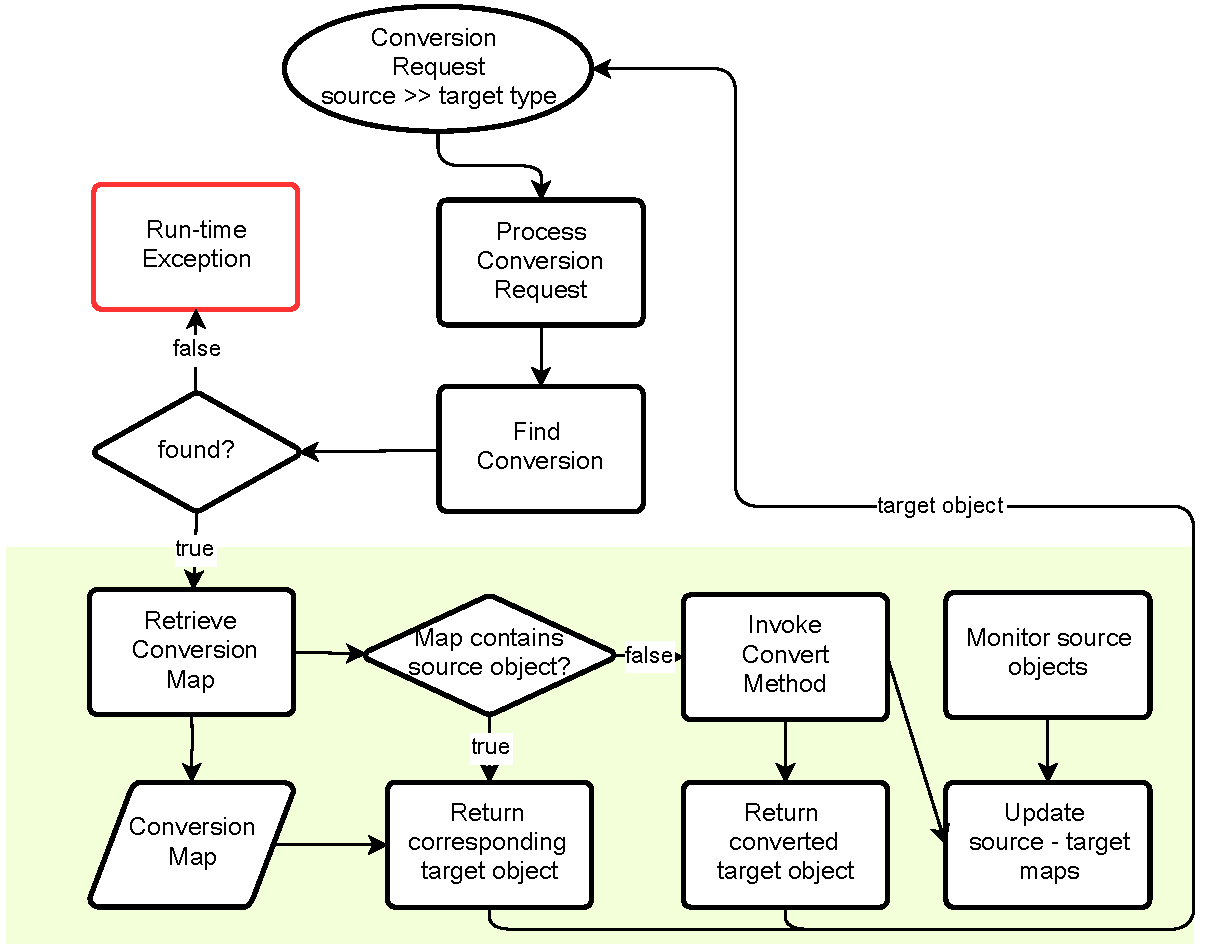
\includegraphics[width=0.8\textwidth]{chapteradapters/runtime2.pdf}
 \caption{The process triggered by a conversion request}
\label{fig:runtime}
\end{figure}

Figure~\ref{fig:runtime} shows how \zamk processes a conversion request. 
For each request the appropriate conversion is found by the \textsf{Find Conversion} process. 
When this process completes successfully, the conversion map of the found conversion is retrieved. 
If the source object already exists in the conversion map, the corresponding target object is retrieved. 
Otherwise a new target object is created by invoking the convert method of the conversion. 
The conversion map is also updated to include the new source--target pair.
Once the desired target object is created or retrieved (in case the given source object is already associated with a target object), it is returned to the owner of the request. 
\zamk runtime is also responsible for managing source--target object pairs, by monitoring the source objects and updating the maps accordingly.

\subsubsection{Initialization}
\label{sec:adapter:loadconvreg}
In order to process conversion requests, \zamk performs a one-time initialization step at the beginning of the run-time which consists of loading the conversion registry and conversion aspect registration. 

\zamk creates a registry of conversion during compile-time (Section~\ref{sec:adapter:convreg}). 
At the beginning of the runtime this registry is loaded by parsing the XML file which contains the conversions. 
As mentioned before the XML file contains data about two kinds of conversions, one-way and two-way.
Each \lstinln{<conversion>} tag is mapped to a \lstinln{Conversion} object, which is the parent type for \lstinln{OneWayConversion} and \lstinln{TwoWayConversion}.
The class structure is shown in Figure~\ref{fig:convclasses}.

\begin{figure}[h]
\centering
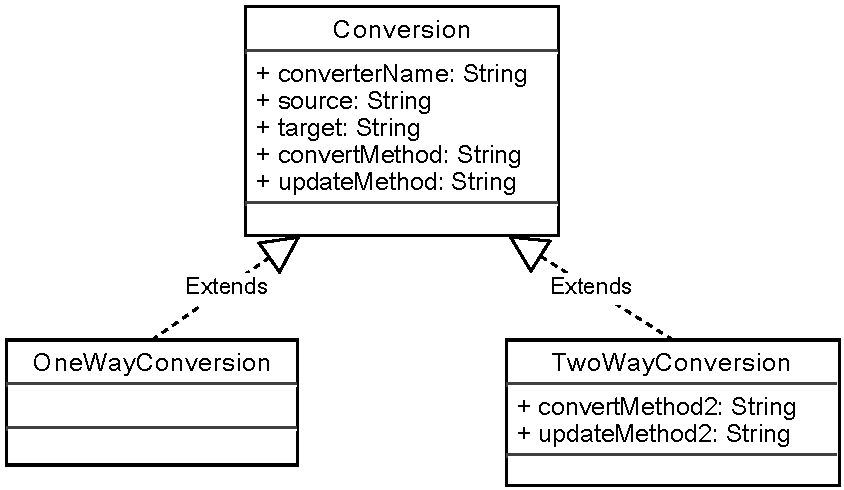
\includegraphics[width=0.6\textwidth]{chapteradapters/ConversionsUML.pdf}
\caption{The run-time \lstinln{Conversion} objects type hierarchy}
\label{fig:convclasses}
\end{figure}

From the conversion data two separate \lstinln{HashMap}s are generated; \lstinln{conversionMap} and \lstinln{sourceMap}.
The \lstinln{conversionMap} is a \lstinln{<String, Conversion>} mapping; the conversions are mapped with their unique ID.  
The \lstinln{sourceMap} is mapping from \lstinln{<Class<?>, ArrayList<String> >}, where \lstinln{Class} represents the source type of the conversion and the \lstinln{ArrayList<String>} is a list of unique IDs of conversion which convert from the source type declared as the key. 
The \lstinln{sourceMap} is constructed to avoid iterating over the whole \lstinln{conversionMap} while searching for a conversion. 

Conversion aspects register their source--target maps during initialization.
This is done by calling the \lstinln{register(String, Map)} method of the \lstinln{ZamkRuntime}. The \lstinln{String} value is the unique ID of the conversion and the \lstinln{Map} is the \lstinln{HashMap} or the \lstinln{BiHashMap} the aspect contains. 
The individual conversion maps are stored in a \lstinln{HashMap} called \lstinln{mapPerConversion}.
Even though the maps are declared and initialized in the conversion aspects, the contents of the maps are managed by the \lstinln{ZamkRuntime}.

\subsubsection{\zamk Conversion Requests}
\label{sec:adapter:convreq}
A conversion request passes on the source object and a desired target type, in return \zamk runtime provides an object which is initialized based on the value of the source object.
The conversion requests are communicated to \zamk with \lstinln{getConvertedValue(Object, Class<?>)} method, which is a static method of \lstinln{ZamkRuntime}.
The pseudo code for \lstinln{getConvertedValue} method is shown in Procedure~\ref{alg:value}. 
The step is to find the suitable conversion for the given input by calling the \lstinln{findConversion} method (line~\ref{findConversion}).
 If this operation is successful, the unique ID of the found conversion is returned and stored in the $uid$ variable). The details of the \lstinln{findConversion} method is discussed in section~\ref{sec:adapter:find}. 
 
Using $uid$ the source--target map for the conversion is retrieved from \lstinln{mapPerConversion} hash-map (line~\ref{getconversionmap}).
This operation works like lazy initialization. 
We check if there is a source--target entry in the conversion map for the given source object, i.e. if the source object has been converted before using this conversion. 
If this is true, then the corresponding target object is retrieved and returned.
Otherwise the request triggers a new conversion, then the \lstinln{invokeConversion} method is called with the $uid$ and the source object to create a new target object. 
The new source--target pair is added to the $map$ and the target object is returned.


\begin{algorithm}
\caption{The \lstinln{getConvertedValue} method}\label{alg:value}
	\begin{algorithmic}[1]
		\Procedure{getConvertedValue}{$source, targetType$}
		\State $sourceType \gets$ \lstinln{source.Class}
		\State $uid \gets$ \lstinln{findConversion(sourceType, targetType)} \label{findConversion}
		\State $map \gets$ \lstinln{mapPerConversion.get(uid)} \label{getconversionmap}
		\If{$source \in map$}
			\State return $map.get(source)$ \label{existingconversion}
		\Else
			\State $target \gets$ \lstinln{invokeConversion(uid, source)} \label{newconversion}
			\State add $(source, target)$ to $map$ \label{addtomap}
			\State \Return $target$
		\EndIf
		\EndProcedure
	\end{algorithmic}
\end{algorithm}

\subsubsection{Finding a Conversion}
\label{sec:adapter:find}
The \lstinln{findConversion} method shown in Procedure~\ref{alg:value} implements an algorithm, which uses type information to find the \emph{closest} conversion among \emph{eligible} conversions for the given source type and the expected target type. 

Given a conversion request from type $X$ to type $Z$, the requirements for an an eligible conversion are as follows:
\begin{enumerate}[{E}-1]
\item The conversion source type is exactly the same as or is a super type of type $X$ and,
\item the conversion target type is exactly the same as or is a sub type of $Z$ type.
\end{enumerate}

The closest conversion is characterized as follows:
\begin{enumerate}[{C}-1]
\item Among eligible conversions its source-type is the closest to the actual type $X$ object given in the conversion request. 
\item Among the eligible conversions with the same source-type proximity, its target-type is the closest to the $Z$ type given in the conversion request.
\end{enumerate}


\begin{figure}[h]
\centering
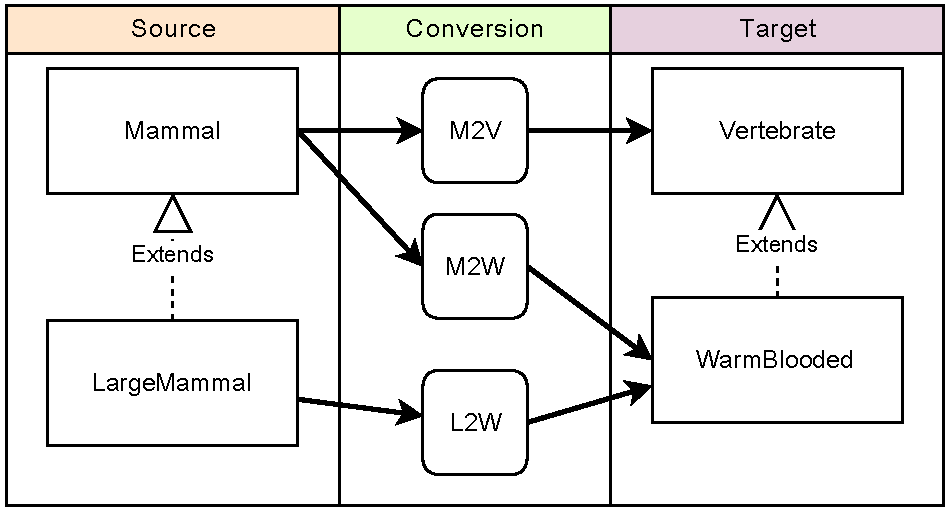
\includegraphics[width=0.8\textwidth]{chapteradapters/animals.pdf}
\caption{Two type hierarchies for representing animals and conversions between them}
\label{fig:animals}
\end{figure}


Let us clarify these descriptions with an example. 
In Figure~\ref{fig:animals} two separate hierarchies that represent different classifications for animals. 
Conversions are defined between the types of these hierarchies.
Consider the conversion request \lstinln{getConvertedValue(largeMammal, Vertebrate.class)}. 
According to our description of the eligible conversions, we can check each conversion to determine if they are in fact eligible.
Starting from the bottom of the figure:
\begin{easylist}[itemize]
& The \lstinln{L2W} conversion converts from \lstinln{LargeMammal} to \lstinln{WarmBlooded}. Since the type of the source object (\lstinln{LargeMammal}) exactly matched the conversion's source type (\lstinln{LargeMammal}) it satisfies E-1, since the target type of this conversion is \lstinln{WarmBlooede} which is a sub-type of \lstinln{Vertebrate}, the conversion also satisfied E-2. Hence we conclude that the conversion is eligible. 
& The conversion \lstinln{M2W} satisfies the E-1 since \lstinln{Mammal} is a super-type of \lstinln{LargeMammal}, it also satisfies E-2 since its target type \lstinln{WarmBlooded} is a sub-type of \lstinln{Vertebrate}.
& Similarly to \lstinln{M2W} the conversion \lstinln{M2V} satisfies E-1 since its source type \lstinln{Mammal} is a super type of \lstinln{LargeMammal} and its target type \lstinln{Vertebrate} is which is exactly the same as the target type given in the conversion request, satisfying E-2.
\end{easylist}
From this analysis we conclude that all three conversions are eligible for this conversion request.

\begin{table}[h]
\centering
\begin{tabular}{ |c|c|c| }
\hline 
Conversion & Source & Target \\
\hline
L2W & 0 & 1 \\
M2W & 1 & 1 \\
M2V & 1 & 0\\
\hline
\end{tabular}
\caption{The type distances of conversion's source--target types to the source--target types given in the conversion request \lstinln{getConvertedValue(mammal, WarmBlooded.class)}}
\label{tab:distance}
\end{table}

To identify the closest conversion, we look at the hierarchical distances of the conversion types to the types given in the conversion request. 
For this example the distances are listed in Table~\ref{tab:distance}.
Even though \lstinln{L2W} and \lstinln{M2V} have the same combined distance, the closest conversion is \lstinln{L2W} since closeness of the source type has priority while deciding on the closest conversion.
The information of the conversion comes from the source object. 
For a conversion to be more accurate, the type of the given source object should be as close as possible to the source type it converts from, i.e the source object should be as specialized as possible. 
That's why the closeness checks prefers the closeness of the source type over the closeness of the target type.


\begin{algorithm}
\caption{The procedure for finding the most suitable conversion}\label{alg:findconv}
	\begin{algorithmic}[1]
		\Procedure{\lstinln{findConversion}}{$sourceType, targetType$}
		\State $eligibles \gets$ empty list
		\State $superTypesSource \gets$ \lstinln{getAllSuperTypes(sourceType)} \label{getsupertypes}
		\While{$superTypesSource.hasNext$} \label{fc:while:b}
		\If{$sourceType \in sourceMap.keySet$} \label{checksourcemap}
			\State $candidates \gets sourceMap.get(source)$ \label{candidates}
			\ForAll{$id \in candidates$} \label{fc:for:b}
			\State $conversion \gets conversionMap.get(id)$ \label{retconv}
			\If{$conversion.getTargetType \subset targetType$} \label{checktarget}
				\State $eligibles.add(id)$
			\EndIf
			\EndFor \label{fc:for:e}
		\Else
			\State $sourceType \gets superTypesSource.next$
		\EndIf
		\EndWhile \label{fc:while:e}

		\If{$eligibles = \emptyset$} \label{eligempty}
		\State Runtime Exception, no conversions found
		\Else
		\State $found \gets$ \lstinln{findClosest(eligibles, sourceType, targetType, superTypesSource)} \label{findclosest}
		\EndIf
		\If{$found > 1$}
		\State \Return \lstinln{resolvePrecedence(found)} \label{resolve}
		\Else
		\State \Return $found(0)$
		\EndIf
		\EndProcedure
	\end{algorithmic}
\end{algorithm}





These operations are implemented in \lstinln{findConversion}; pseudo code is shown in Procedure~\ref{alg:findconv}.
The procedure starts by creating an empty list named $eligibles$ which will contain the eligible conversions.
In order to determine these conversions, we first need to find the super types of the source  type by walking their type hierarchy. 
This is done by the method \lstinln{getAllSuperTypes} which uses reflection to populate the full set of super types (classes and interfaces) of a given type. 
On line~\ref{getsupertypes} this method is called and the returned list is stored in $superTypeSource$. 
Note that when the \lstinln{java.lang.Object} is passed as an argument to this method, it returns a list that contains a set that contains the single element \lstinln{java.lang.Object}.

The while loop (lines~\ref{fc:while:b}--~\ref{fc:while:e}) iterates over the $superTypeSource$ set and checks if that source type is associated with any conversions; in the \lstinln{if} statement on line~\ref{checksourcemap} checks if $sourceMap$'s key set contains the $sourceType$.
When this expression evaluates to true, we retrieve the candidate conversions from the $sourceMap$ and store them into the list $candidates$ (line~\ref{candidates}).
The $candidates$ list contains the conversion IDs that converts from the $sourceType$.
The conversions pointed by $candidates$ only satisfy the source type criteria of an eligible conversion, therefore we still need to check the target types of these conversions to detect if they are indeed eligible.
This detection is done in the for loop on lines~\ref{fc:for:b}--~\ref{fc:for:e}.
For each unique id in the list $candidates$, we retrieve the corresponding conversion from the $conversionMap$ (line~\ref{retconv}) and store it into the variable $conversion$. 
Then we check if the target type of this $conversion$ is a sub-type from the $targetType$ passed to the conversion request (line~\ref{checktarget}). 
If this expression is true then we add the id of the $conversion$ to the list of $eligibles$.

When the if statement on line~\ref{checksourcemap} evaluates to false, then we set the variable $sourceType$ to the next element in $superTypesSource$ and reiterate the process until there are no more elements left in $superTypesSource$.
At the end of this iteration, we obtain a list of eligible conversions stored in $eligibles$.

The next operation is to find the closest conversion from this list. 
First we check if the list $eligibles$ is empty (line~\ref{eligempty}); if it is an empty list then we throw a run-time exception, indicating there are no suitable conversions found for the given source and target types.
If the list is non-empty then we invoke the method \lstinln{findClosest} (line~\ref{findclosest}) and store the returned conversion id values in the variable $found$. 
It is possible that there are more than one equally close conversions for a given request, if this is the case we invoke to \lstinln{resolvePrecedence} method (line~\ref{resolve}) and return the value obtained from this method. 
If the \lstinln{resolvePrecedence} method cannot resolve the ambiguity in the $found$ list then it throws a run-time exception, indicating there is not enough information to resolve the precedence.
If the \lstinln{findClosest} method returns a single conversion then we simply return the first element of the list $found$.

\paragraph{\lstinln{getAllSuperTypes} method} This is a utility method which returns the super-types of a type. We use reflection to walk the type hierarchy of the given type. The source code for this method is shown in Listing~\ref{lst:allsupertypes}.
On line~\ref{lst:list} we create an empty list which will hold the super types of \lstinln{sourceType}.
Then we add the \lstinln{sourceType} to this list as the first element (line~\ref{lst:list}). 
On line~\ref{lst:super}, by using the reflection method \lstinln{getSuperClass} we store the super type of \lstinln{sourceType} to the variable \lstinln{superType}. 
The reflective method \lstinln{getInterfaces} is used to return the interface a type implements, which is called on line~\ref{lst:itc:b}. These interface are added to the list \lstinln{sourceTypeHier} by iterating over the list \lstinln{itc}.
The while loop shown on lines~\ref{lst:while:b}--~\ref{lst:while:e} is only executed if the variable \lstinln{superType} is not \lstinln{Object}, since that is the root type for all objects in Java.
Inside the while loop the same operations described above are performed until the next source type is \lstinln{java.lang.Object} which is added to the list after the loop terminates.
Finally the \lstinln{sourceTypeHier} list is returned. 

\begin{lstlisting}[float, caption={The source code for the \lstinln{getAllSuperTypes} method}, label={lst:allsupertypes}]
private static List<Class<?>> getAllSuperTypes(Class<?> sourceType) throws ClassNotFoundException {
	List<Class<?>> sourceTypeHier = new ArrayList<Class<?>>(); ~\label{lst:list}~
	sourceTypeHier.add(sourceType); ~\label{lst:add}~
	Class<?> superType = sourceType.getSuperclass(); ~\label{lst:super}~
	Class<?>[] itc = superType.getInterfaces(); ~\label{lst:itc:b}~
	for(int i=0; i<itc.length; i++)
	{
		sourceTypeHier.add(itc[i]);
	}~\label{lst:itc:e}~
	while (!superType.getName().equals("java.lang.Object")) { ~\label{lst:while:b}~
		sourceTypeHier.add(superType);
		itc = superType.getInterfaces();
		for(int i=0; i<itc.length; i++)
		{
			sourceTypeHier.add(itc[i]);
		}
		superType = superType.getSuperclass();
	}~\label{lst:while:e}~
	sourceTypeHier.add(Class.forName("java.lang.Object"));
	return sourceTypeHier;
}
\end{lstlisting}

\paragraph{\lstinln{findClosest} method} This method find the closest conversion from the list of eligible conversions. 
In order to perform this task, the method takes the eligibles list, source and target types and the lists of their super types as an argument. 
The method creates the table shown in Table~\ref{tab:distance} for each eligible conversion, and decides on the closest according to the closest conversion criteria given at the beginning of this section. 
\TODO{pseudo code}

\paragraph{\lstinln{resolvePrecedence} method} When \lstinln{findClosest} method finds multiple equally close conversion for a conversion request, the \lstinln{resolvePrecedence} method is invoked.
The task of this method is to process the precedence information given during compile-time and decide which of the conversions should be applied to a conversion request.
\TODO{pseudo code}

\subsubsection{Target Object Creation and Retrieval}
In section~\ref{sec:adapter:convreq} we have mentioned the steps taken after a conversion is found.
In this section we will discuss these steps in detail. 

\begin{algorithm}
\caption{Partial view of the \lstinln{getConvertedValue} method}\label{alg:value2}
	\begin{algorithmic}[1]
		\Procedure{getConvertedValue}{$source, targetType$}
		...
		\State $map \gets$ \lstinln{mapPerConversion.get(uid)} \label{getconversionmap2}
		\If{$source \in map$}
			\State return $map.get(source)$ \label{existingconversion2}
		\Else
			\State $target \gets$ \lstinln{invokeConversion(uid, source)} \label{newconversion2}
			\State add $(source, target)$ to $map$ \label{addtomap2}
			\State \Return $target$
		\EndIf
		\EndProcedure
	\end{algorithmic}
\end{algorithm}


We show a partial pseudo code of the \lstinln{getConvertedValue} in Procedure~\ref{alg:value2}.
When \lstinln{findConversion} method returns a conversion id, we use it to retrieve the map for that conversion. 
Then we check if the map contains the $source$ object, if it does we return the target object, associated with this $source$. 
This operation is called target object retrieval. 
By having this operation, we ensure that the state of a conversion is preserved, similar to an object adapter inferring its state from its adaptee. 

If the $source$ object was not converted before with found conversion, we need to create a new source--target pair.
To do this we must call the \lstinln{invokeConversion} method, which reflectively invokes the convert method of the found conversion.
The source code for this method is given in listing~\ref{lst:invokeconv}.
The argument \lstinln{uid} is used to retrieve the conversion from the \lstinln{conversionMap} (line~\ref{lst:getconv}). A \lstinln{Conversion} object contains the fully-qualified name of the converter it is contained in and the names of the convert and update methods. 
We first create a \lstinln{Class} object for the converter that contains the \lstinln{conversion} (line~\ref{lst:getconvclass}). 
After constructing an array for argument types of the convert method (line~\ref{lst:args}), the convert method for the \lstinln{converter} is loaded from the \lstinln{Class converter} (line~\ref{lst:method}). 
The retrieved method is invoked by calling the \lstinln{invoke} method and passing on the argument \lstinln{source} (line~\ref{lst:invoke}).
The result of the method invocation is stored in the variable \lstinln{trgt} which was initially null and returned. 


\begin{lstlisting}[float, caption={The \lstinln{invokeConversion} method which reflectively invokes the convert method of a given conversion}, label={lst:invokeconv}]
public static <T, U> T invokeConversion(String uid, U source) {
	T trgt = null;
	Conversion conversion = conversionMap.get(uid); ~\label{lst:getconv}~
	Class converter = Class.forName(conversion.getConverterName()); ~\label{lst:getconvclass}~
	Class[] argTypes = new Class[] { source.getClass() }; ~\label{lst:args}~
	Method convert = converter.getDeclaredMethod(conversion.getConvertMethod(), argTypes); ~\label{lst:method}~
	trgt = (T) convert.invoke(null, source); ~\label{lst:invoke}~
	return trgt;
}
\end{lstlisting}


\subsubsection{Object Synchronization}
\label{sec:adapter:sync}
The source--target pairs kept in the conversion maps are maintained by conversion aspects. 
We have previously discussed the structure and the members of these aspect in section~\ref{sec:adapter:codegen}.
A conversion adapter contains a pointcut (\lstinln{updateObserverThis}) which monitors all of the changes made to the objects of source type.
When this pointcut matches, the changed object is bound. 
The after advice that uses this pointcut, looks at its source--target map to check if the map contains the bound object as a key. 
If this is the case, then the corresponding target object is updated by creating a new object of target type and passing the values of the newly created object to the existing target object. 
The copying of the values is performed by the update method of the conversion.

\subsubsection{Run-time API}
\zamk run-time API offers two overloaded methods to access its functionality.

\begin{easylist}[itemize]
& \lstinln{getConvertedValue(U source, Class<T> targetType)} : This method invokes the fully-automated functionality of \zamk. 
The run-time steps mentioned in the sections before take place, and the converted value is returned.
& \lstinln{getConvertedValue(U source, Class<T> targetType, String using)} : Calling this method is equivalent to adding a \lstinln{using} clause in \gluer. 
The \lstinln{String} argument should be the fully-qualified name of the conversion. 
In this method the \lstinln{findConversion} is not called.
\end{easylist}
\TODO{expand this section}

\section{Related Work}
\section{Conclusion}

